%%% Layout
\documentclass[11pt]{article}
\usepackage{fancyhdr}
\pagestyle{headings}
\usepackage{fullpage}


%%% Math
\usepackage{amsmath}
\usepackage{amssymb}
\usepackage{esint}
\usepackage{indentfirst}
\usepackage{gensymb}
\usepackage{mathtools}
\usepackage{listings}

%%% Graphics
\usepackage{graphicx}
\usepackage[subrefformat=parens,labelformat=parens]{subfig}

%%% Bibliography
\usepackage[verbose]{cite}
\bibliographystyle{unsrt}
\usepackage{url}

%%% Mark-up
\usepackage{color} % text color
%\usepackage{soul} % mark up effects
%\usepackage{todonotes}

%%% Title
\lhead{AA 543 Winter 2017 HW\#5}
\chead{}
\rhead{Crews \& Thomas, HW\#5}
\cfoot{\thepage}
\title{AA 543 Winter 2017 HW\#5}
\author{D. W. Crews and W.R. Thomas}
\date{\today}

\begin{document}
\maketitle

\section{Definition of problem}
Solve numerically the 2D Euler equations for the transonic flow over a NACA 0012 airfoil using the Jameson scheme (Jameson et al., AIAA 1981).  

\noindent The following conditions are given:
\begin{itemize}
	\item Angle of attack $\alpha = 0 \deg$
	\item Free-stream Mach number $M_\infty = 0.85$
\end{itemize}

\noindent These further free-stream conditions are defined given an altitude of 10 km as per the Standard Atmosphere Table 1976.
\begin{itemize}
	\item $\gamma \approx 1.4$
	\item Density $\rho_\infty = 0.414 \; \text{kg/m}^3$ 
	\item Temperature $T_\infty = 223.3 $ K
	\item Pressure $p_\infty = 26.5 $ kPa
	\item Sound speed $c_\infty = \sqrt{\gamma \frac{p_\infty}{\rho_\infty}} = 299 \approx 300 $ m/s
	\item Velocity $|\vec{u}_\infty| = M_\infty c_\infty = 255$ m/s. 
	
	Therefore $u_\infty = |\vec{u}_\infty| \cos\alpha = 255$ m/s and  $v_\infty = |\vec{u}_\infty| \sin\alpha = 0$ m/s.
	\item Energy $E_\infty = e + \frac{|\vec{u}_\infty|^2}{2}$ where $e = \frac{p_\infty}{\rho_\infty (\gamma -1)} $. The free-steam energy is then $E_\infty = 193 $ J
\end{itemize}

\section{Implementation of the numerical scheme}
	\subsection{Grid}
	The grid was created by Daniel Crews for Homework \#3.
	
	Because the grid is not a uniform rectangular grid, cell areas and cell wall normals will have values for each cell. To facilitate calculations, these quantities are calculated during the initialization of the simulation and stored in vectors.  The cell vertices (as provided by the grid file) are indicated by $\vec{X}_{i,j}=[X_{i,j},Y_{i,j}]$, and the cell centers by $\vec{x}_{i,j}=[x_{i,j},y_{i,j}]$.  See Figure \ref{grid_nameing} for naming and indexing convention used in this implementation.
		\begin{figure}[ht!]
			\centering
			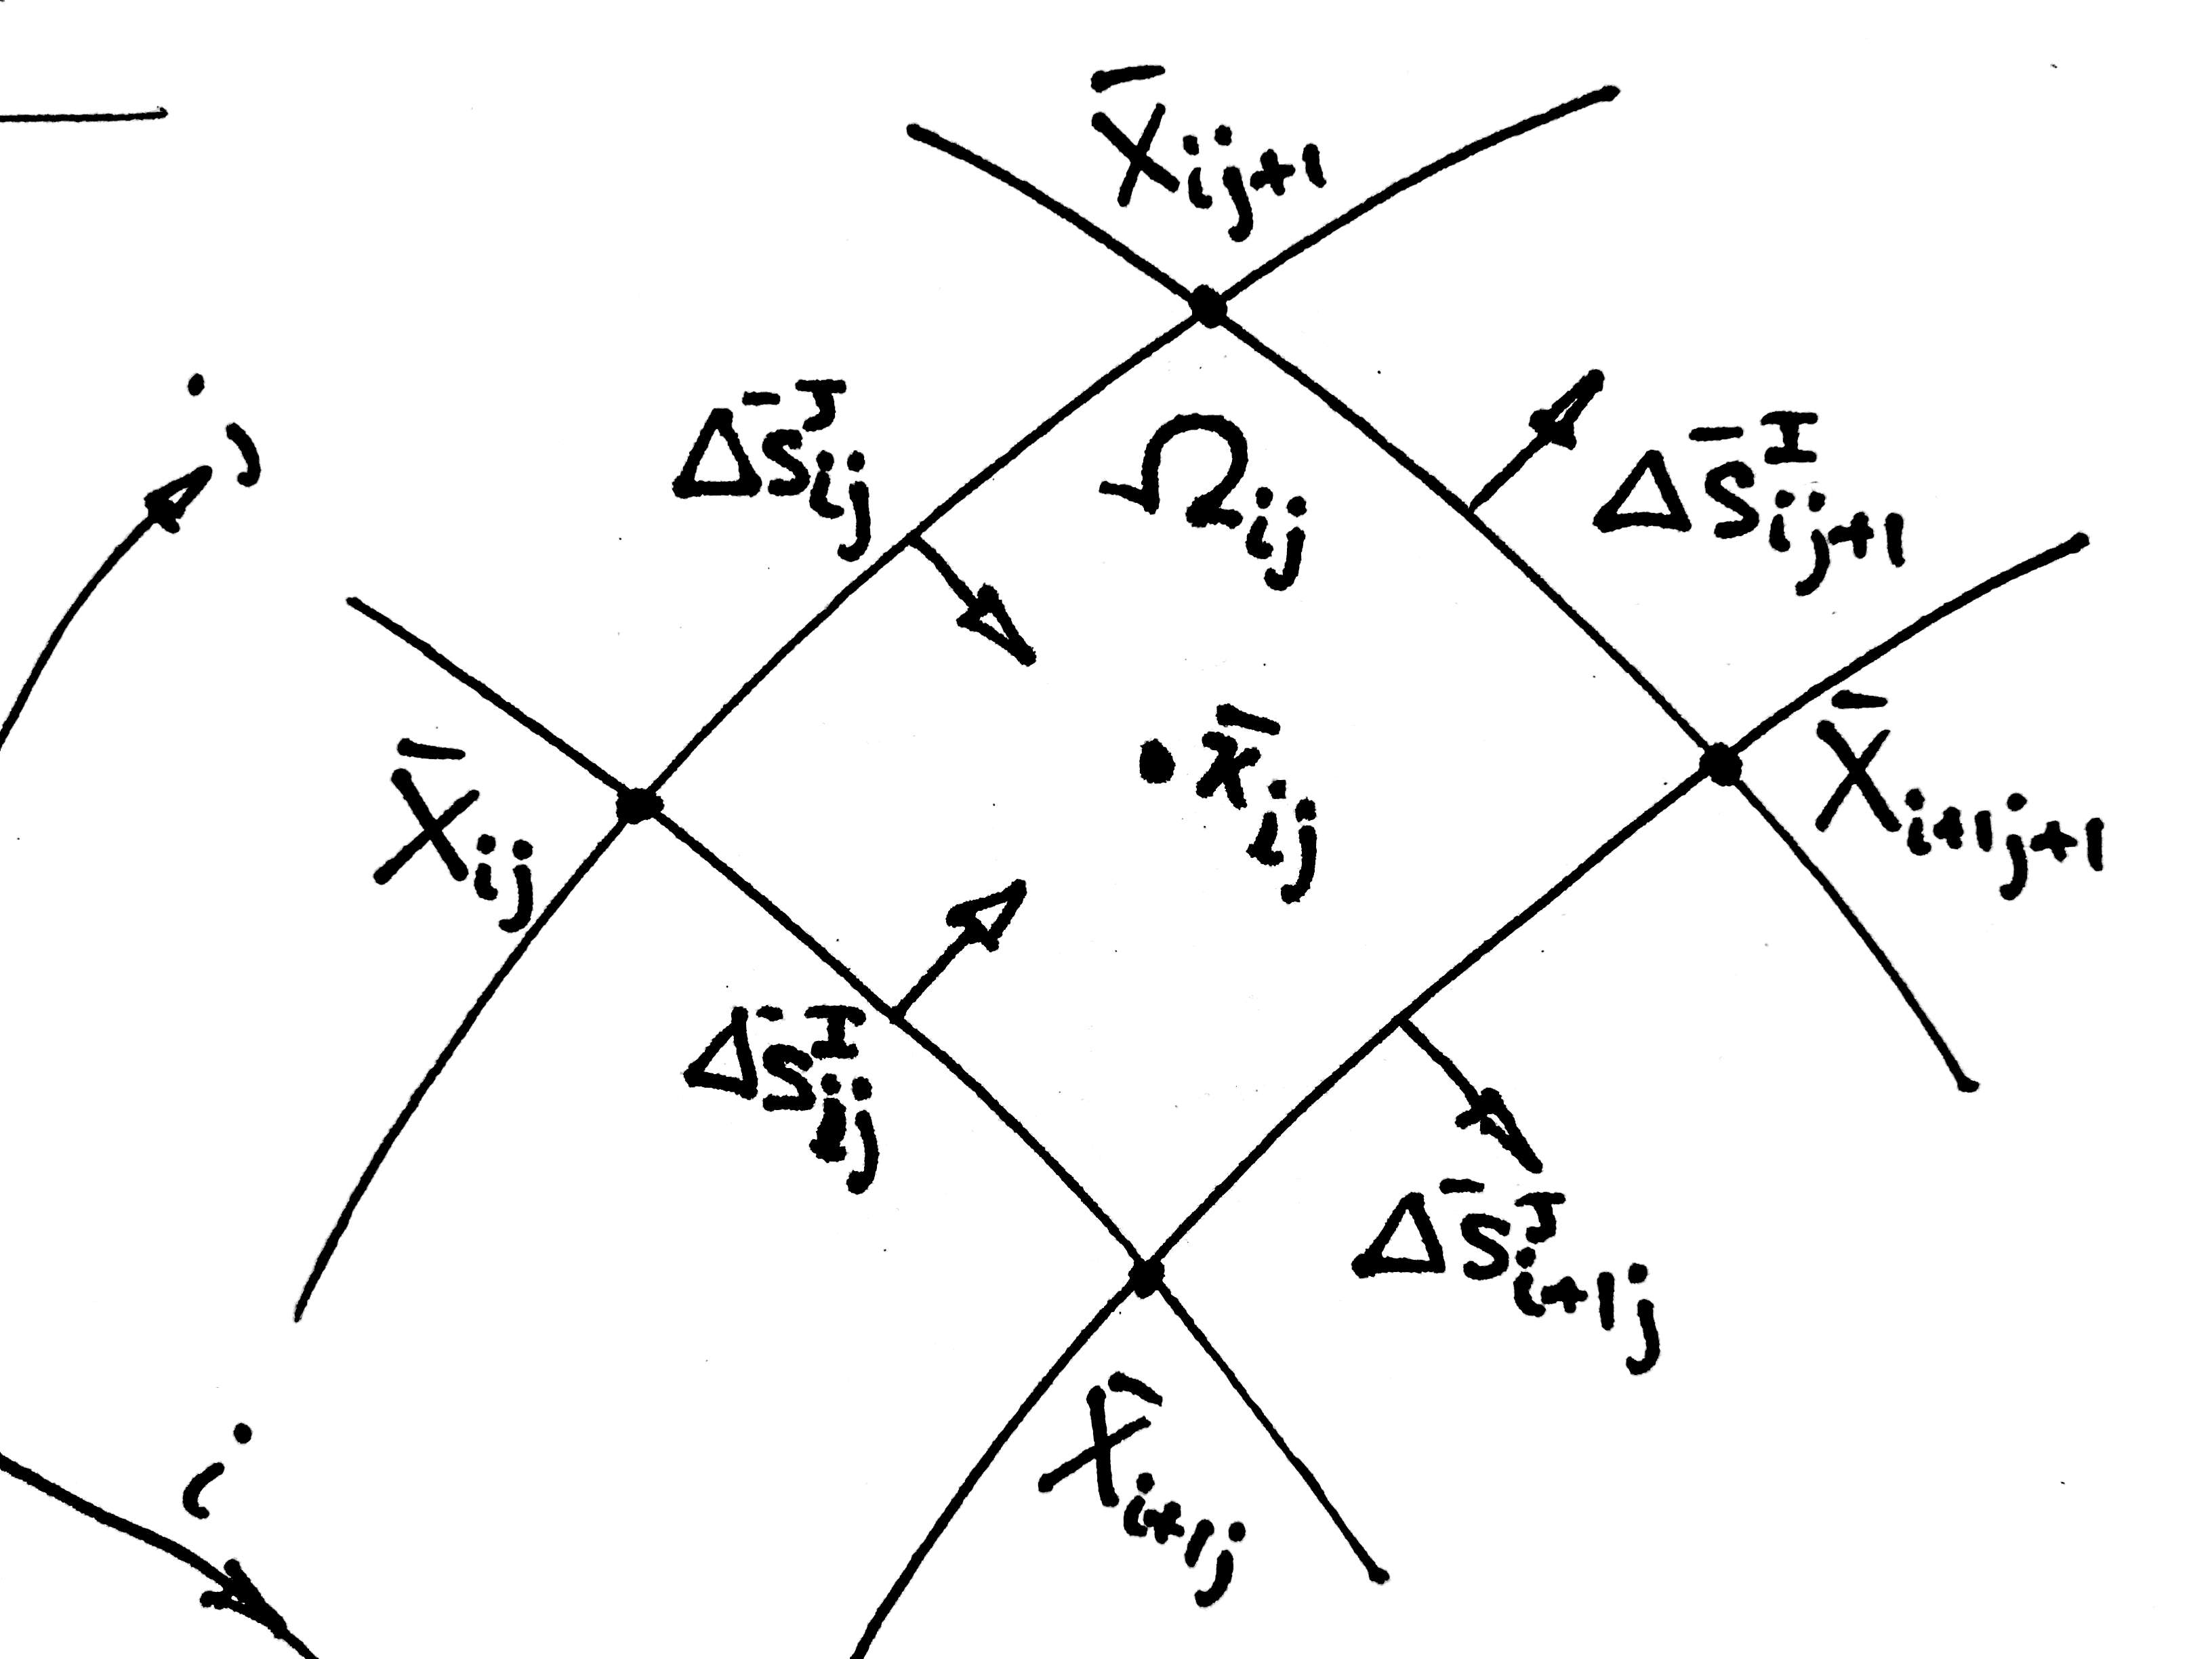
\includegraphics[width=4in]{figures/grid_naming_conv.jpg}
			\caption{Grid naming and indexing convention.}
			\label{grid_nameing}
		\end{figure}
		
	\subsubsection*{Cell centers}
	Cell centers are found by a simple average of cell vertices.
		\begin{align}
		&x_{i,j} = \frac{1}{4} (X_{i,j} + X_{i+1,j} + X_{i,j+1} + X_{i+1,j+1}) \\
		&y_{i,j} = \frac{1}{4} (Y_{i,j} + Y_{i+1,j} + Y_{i,j+1} + Y_{i+1,j+1})
		\end{align}
	
	\subsubsection*{Cell areas}
	The cell areas is computed as one half the absolute value of the cross product of the diagonals of the cell:
		\begin{align}
		\Omega_{i,j} &= \frac{1}{2} \left|(\vec{X}_{i+1,j} - \vec{X}_{i,j+1}) \times (\vec{X}_{i+1,j+1} - \vec{X}_{i,j})\right| \\
		& = \frac{1}{2} \left| \begin{bmatrix}
		X_{i+1,j} - X_{i,j+1} \\ Y_{i+1,j} - Y_{i,j+1}
		\end{bmatrix} \times \begin{bmatrix}
		X_{i+1,j+1} - X_{i,j} \\ Y_{i+1,j+1} - Y_{i,j}
		\end{bmatrix} \right| \\
		& = \frac{1}{2} \left| (X_{i+1,j} - X_{i,j+1})(Y_{i+1,j+1} - Y_{i,j}) - (X_{i+1,j+1} - X_{i,j})(Y_{i+1,j} - Y_{i,j+1}) \right|
		\end{align}
		
	\subsubsection*{Cell wall normals}
	We have chosen to compute cell normals in their global orientation (see Figure \ref{grid_nameing}). We store two sets of normals arrays: $\Delta \vec{s}_{i,j}^I$ contain the $x$ and $y$ components of the cell normals of walls whose vertices increase with $i$, and $\Delta \vec{s}_{i,j}^J$ contain the $x$ and $y$ components of the cell normals of walls whose vertices increase in $j$. 
		\begin{align}
		&\Delta \vec{s}_{i,j}^I = (Y_{i+1,j} - Y_{i,j})\hat{x} - (X_{i+1,j} - X_{i,j})\hat{y} \\
		&\Delta \vec{s}_{i,j}^J = (Y_{i,j+1} - Y_{i,j})\hat{x} - (X_{i,j+1} - X_{i,j})\hat{y} 
		\end{align}
	
	\subsubsection*{Unit normal \& unit tangent vectors}
	Unit normals and unit tangent vectors are used in implementing boundary conditions, and can be found by normalizing the cell wall normals by their length (for the unit normal), and a 90 \degree CW rotation (for the unit tangent).  For the outer boundary they will be
		\begin{align}
		&\hat{n}_{i,M} = -\frac{\Delta s_{i,M}^I}{|\Delta s_{i,M}^I|} = \frac{(Y_{i+1,M} - Y_{i,M})\hat{x} - (X_{i+1,M} - X_{i,M})\hat{y}}{(Y_{i+1,M} - Y_{i,M})^2 + (X_{i+1,M} - X_{i,M})^2} \\
		&\hat{\ell}_{i,M} =  R(90 \degree) \hat{n}_{i,M} = \begin{bmatrix} 0 & 1 \\ -1 & 0 \end{bmatrix} \hat{n}_{i,M}
		\end{align}
	For the airfoil boundary they are
		\begin{align}
		&\hat{n}_{i,0} = -\frac{\Delta s_{i,0}^I}{|\Delta s_{i,0}^I|} = \frac{(Y_{i+1,0} - Y_{i,0})\hat{x} - (X_{i+1,0} - X_{i,0})\hat{y}}{(Y_{i+1,0} - Y_{i,0})^2 + (X_{i+1,0} - X_{i,0})^2} \\
		&\hat{\ell}_{i,0} =  R(90 \degree) \hat{n}_{i,0} = \begin{bmatrix} 0 & 1 \\ -1 & 0 \end{bmatrix} \hat{n}_{i,0}
		\end{align}
	\subsection{Normalization (??)}
	(Normalize to free-stream values?)
	
	\subsection{Initial conditions}
	Initial conditions will be the same as the free-stream values, for all points in the domain.
		\begin{align}
		U_{i,j}^0 = \begin{bmatrix}
		\rho_\infty \\ \rho_\infty u_\infty \\ \rho_\infty v_\infty \\ \rho_\infty E_\infty
		\end{bmatrix}
		\end{align}
	
	\subsection{Boundary conditions}
		\subsubsection{Outer boundary}
		The outer boundary conditions will be a subsonic ($M_\infty=0.85$) laminar flow in the $\hat{x}$ direction. To maintain a laminar, physically consistent flow across these boundaries, several conditions must be enforced:
			\begin{enumerate}
				\item Riemann invariants $R_n^\pm$ are constant along path $\vec{u} + c\hat{n}$.
				\item Riemann invariant $u_\ell$ is constant in direction $\hat{n}$.
				\item Enthalpy $H$ or entropy $S$ is constant (conservation of energy in a steady flow).
			\end{enumerate}
			
		 Because the boundary is circular, and some regions will be inflow, and some outflow, the information used to satisfy the conditions above at the ghost cells will either come from given free-stream values (physical conditions) or from the interior (numerical boundary conditions).  The boundary condition applied will depend on the orientation of the boundary cell unit normals $\hat{n}$ (by convention pointing in) to the fluid velocity $\vec{u}$.
		
		\subsubsection*{Subsonic inflow, $\vec{u} \cdot \hat{n} > 0$}
		In the subsonic inflow case, $R_{nB}^+$ (where $B$ indicates the ghost cell) is coming from the exterior (physical boundary condition), and $R_{nB}^-$ is coming from the interior (numerical boundary condition). 
			\begin{align}
			&R_{nB}^+ = u_{nB} + \frac{2c_B}{\gamma - 1} = R_{n\infty}^+ = u_{n\infty} + \frac{2c_\infty}{\gamma - 1} \\
			&R_{nB}^- = u_{nB} - \frac{2c_B}{\gamma - 1} = R_{nI}^- = u_{nI} - \frac{2c_I}{\gamma - 1}
			\end{align}
		Where $I$ indicates the interior. We can now write the following, which can be used to determine values in boundary cells:
			\begin{align}
			&u_{nB} = \frac{R_{nB}^+ + R_{nI}^-}{2} \\
			&u_{\ell B} = u_{\ell\infty} \\
			&c_B = (R_{nB}^+ - R_{nI}^-) \frac{\gamma - 1}{4} \\
			&H_{B} = H_\infty 
			\end{align}
		Written in terms of our grid parameters, primitive variables, and free stream constants, this looks like: 
			\begin{align}
			&\vec{u}_{i,M+1} \cdot \hat{n}_{i,M} = \frac{R_{i,M+1}^+ \cdot \hat{n}_{i,M} + R_{i,M}^- \cdot \hat{n}_{i,M}}{2} \\
			&\vec{u}_{i,M+1} \cdot \hat{l}_{i,M} = \vec{u}_\infty \cdot \hat{\ell}_{i,M} \\
			&c_{i,M+1} = (R_{i,M+1}^+ \cdot \hat{n}_{i,M} - R_{i,M}^- \cdot \hat{n}_{i,M}) \frac{\gamma - 1}{4} \\
			&E_{i,M+1} + \frac{p_{i,M+1}}{\rho_{i,M+1}}= E_\infty + \frac{p_\infty}{\rho_\infty} 
			\end{align}
		And finally we can prescribe our conserved variables in our ghost cells as:
			\begin{align}
			U_{i,M+1} = \begin{bmatrix}
			\rho \\ \rho u \\ \rho v \\ \rho E
			\end{bmatrix} = 
			\begin{bmatrix}
			\rho_{i,M} \\
			\rho_{i,M}(...  + \vec{u}_\infty \cdot \hat{\ell}_{i,M}) \cdot \hat{x} \\
			\rho_{i,M}(...  + \vec{u}_\infty \cdot \hat{\ell}_{i,M}) \cdot \hat{x} \\
			\rho_{i,M+1} \left( E_\infty + \frac{p_\infty}{\rho_\infty} - \frac{p_{i,M+1}}{\rho_{i,M+1}} \right)
			\end{bmatrix}
			\end{align}
		{\color{red} Still need to define density or pressure!!!!}
		
		\subsubsection*{Subsonic outflow, $\vec{u} \cdot \hat{n} < 0$}
		Subsonic outflow has the same requirements as subsonic inflow, except that now
			\begin{align}
			&R_{nB}^+ = -|u_{nB}| + \frac{2c_B}{\gamma - 1} = R_{n\infty}^+ = -|u_{n\infty}| + \frac{p_\infty}{\rho_\infty c_\infty} \\
			&R_{nB}^- = -|u_{nB}| - \frac{2c_B}{\gamma - 1} = R_{nI}^- =u_{nI} - \frac{2c_I}{\gamma - 1}
			\end{align}
		{\color{red} Not sure why in the interior/exterior are not reversed here from the inflow boundary, but is how it is written in the notes. Will see if it causes problems in the implementation.}
		\subsubsection{Air foil boundary}
		Along the air foil, there will be a free slip boundary, and normal velocity $u_n = 0$. Density, pressure, energy and transverse velocity will be extrapolated linearly from the interior.
			\begin{align}
			U_{i,0-1} = \begin{bmatrix}
			\tilde{\rho} \\ \tilde{\rho} \tilde{\tilde{u}} \\ \tilde{\rho} \tilde{\tilde{v}} \\ \tilde{\rho} \tilde{E}
			\end{bmatrix}_{i,0-1}
			\end{align}
		Where the $\tilde{\tilde{u}}$ and $\tilde{\tilde{v}}$ contain the extrapolated transverse velocity and an equal but opposite normal velocity to the cell inside the boundary
			\begin{align}
			\tilde{\tilde{u}}_{i,-1} = (-[u\hat{x} + v\hat{y}]_{i,0} \hat{n}_{i,0} + [\tilde{u}\hat{x} + \tilde{v}\hat{y}]_{i,-1} \hat{\ell}_{i,0}) \cdot \hat{x} \\
			\tilde{\tilde{v}} _{i,-1} = (-[u\hat{x} + v\hat{y}]_{i,0} \hat{n}_{i,0} + [\tilde{u}\hat{x} + \tilde{v}\hat{y}]_{i,-1} \hat{\ell}_{i,0}) \cdot \hat{y}
			\end{align}
		The unit vectors $\hat{n}$ and $\hat{\ell}$ are defined in Section 2.1. For extrapolated values in ghost cells for density, transverse velocity, and energy, the following equation is used (here $q$ is an arbitrary scalar variable)
			\begin{align}
			\tilde{q}_{i,-1} = ax_{i,-1} + by_{i,-1} + c
			\end{align}
		Where the coefficients $a, b$ and $c$ are found using a linear least squares fit on $q_{i,0}, q_{i,1}$ and $q_{i,2}$.
		
		\subsubsection{Boundaries along O-mesh slice}
		These boundaries will be periodic. There is no need for ghost cells as
			\begin{align}
			U_{-1,j} = U_{N-1,j}; \quad U_{N+1,j} = U_{0,j}
			\end{align}
	\subsection{Spacial discretization of 2D Euler equations with Jameson scheme}
	(copy from notes)
	
	\subsection{Temporal discretization with Runge-Kutta 4 step time integration scheme}
	(copy from notes)
	
	\subsection{Determining convergence to steady state condition}

\section{Results \& Analysis}	
		
	
\subsection{Bonus}

	
	

\pagebreak
\appendix
\section{Code}
	\subsection{2d\_euler\-jameson.cc}
%		\lstinputlisting[language=C++]{../code/2d_euler_jameson.cc}
		
	

\end{document}

